\documentclass{article}
\usepackage{graphicx}
\newcommand{\documentname}{paper~}
\newcommand{\match}{{\tt match}~}
\newcommand{\apj}{ApJ}
\newcommand{\apjs}{ApJS}
\newcommand{\apjl}{ApJL}
\newcommand{\aj}{AJ}
\newcommand{\mnras}{MNRAS}
\newcommand{\mnrassub}{MNRAS accepted}
\newcommand{\aap}{A\&A}
\newcommand{\aaps}{A\&AS}
\newcommand{\araa}{ARA\&A}
\newcommand{\nat}{Nature}
\newcommand{\physrep}{PhR}
\newcommand{\pasp}{PASP}
\newcommand{\pasj}{PASJ}
\title{Spheres}
\author{Jaime E. Forero-Romero}
\begin{document}
\maketitle
\begin{abstract}

Gravity is the dominant force shaping the spatial distribution of galaxies in
the Universe. Under the assumption of homogeneity and isotropy of the Universe
beyond a certain physical scale one can usually approximate the local
kinematic evolution of galaxy by the matter distribution below that
homogeneity scale. In this letter we show that if the matter
distribution is composed by a discrete set of points then, due to
statistical fluctuations, the influence of matter has a measurable
effect at all scales. Our results are based on straightforward
analytical considerations, monte-carlo realizations and the analysis
of cosmological N-body simulations. We discuss the implications of
these results in the interpretation of the peculiar motion of our
galaxy. We suggest possible cosmological tests of these ideas for
future observational facilities. 



\end{abstract}

1. Of all the fundamental forces gravity plays the dominant role in
defining the large scale structure of the Universe. From very
homogeneous conditions gravitational instability drives the emergence
of a web-like pattern. The influence of
matter beyond that scale can be discarded on the grounds that
the net gravitational force inside an homogeneous spherical
shell is zero. [Inhomogeneity, Kirchoff's theorem] [...]



2. Large galaxy surveys help us to define different physical scales for
homogeneity [...]


3. We consider first a simple phenomenological model where matter is
homogeneously distributed over the surface of a sphere of radius
$R$. This distribution consists of a set of $N_p$ point masses with mass
$m$. Under these conditions the total force, $F_{\rm T}$, at the
center of that spherical distribution can be expressed in terms of the
force $F_{\rm m}(R)$ produced by a single point mass located at a
position  $R$ as follows:  

\begin{equation}
F_{\rm T } = N_p^{1/2} F_{\rm m} (R),
\end{equation}
%
a results that can be explained analytically
\cite{Chandra43,Carati2008}. In Figure \ref{fig:sphere_surface} we
show the results of a simple Monte Carlo simulation where $N_p$
particles are located over the surface sphere of radius $R$, the total force per
unit mass on a test particle, $F_{\rm T}$, is then expressed as a
multiple of $F_{m}(R)=Gm_p/R^2$. This shows how the analytical
expectation is a good approximation to the results obtained through
MonteCarlo simulations.




\begin{figure}
\begin{center}
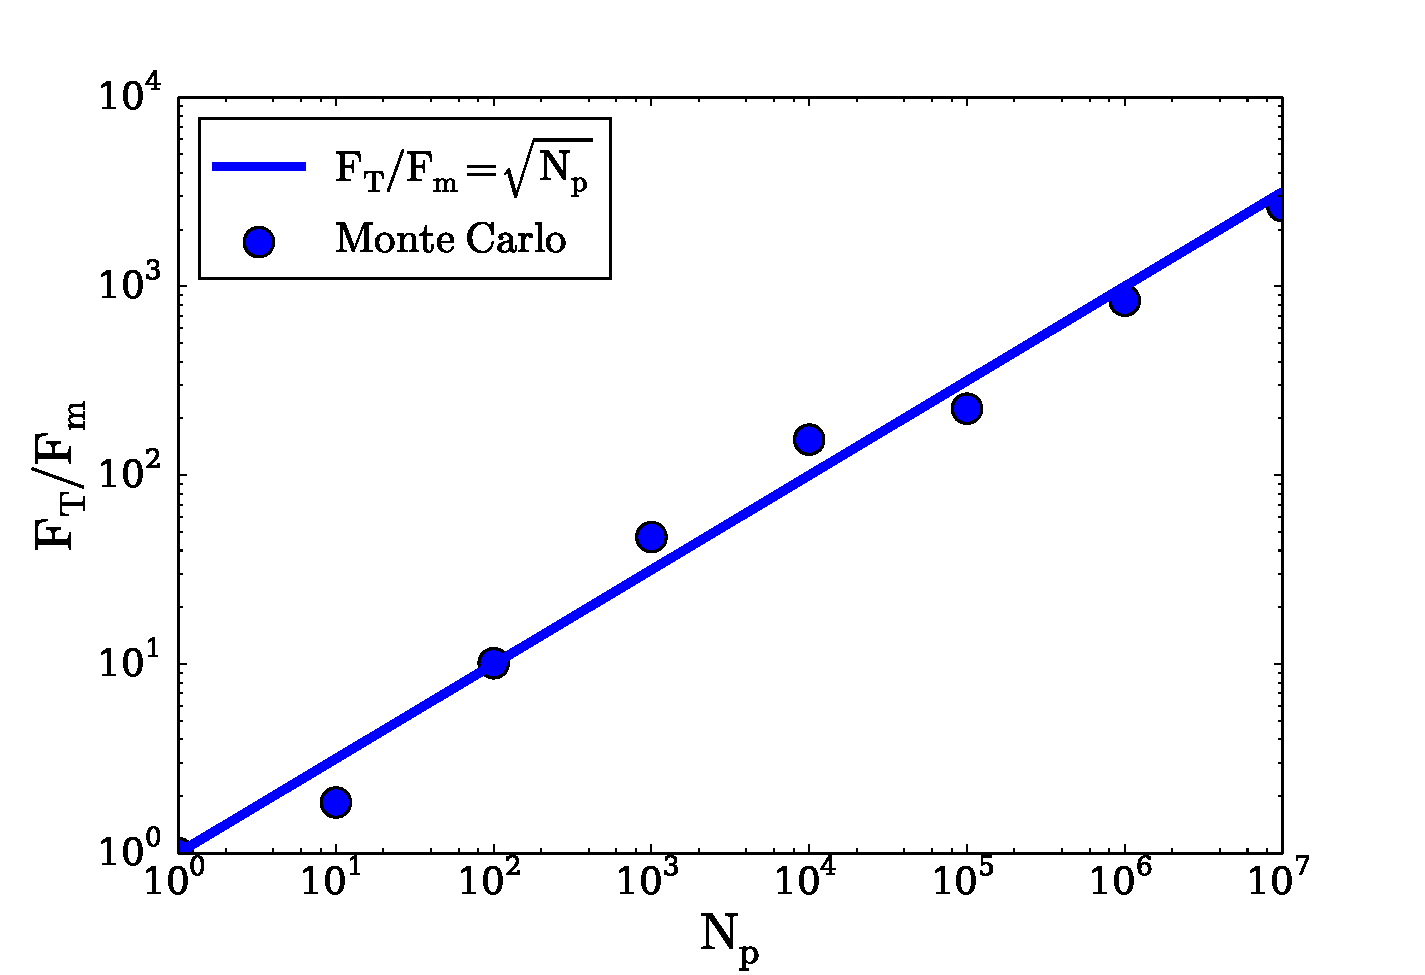
\includegraphics[width=0.8\linewidth,angle=0]{spheres_surface.pdf}
\caption{Norm of the total force per unit mass, $F_{T}$, produced by a distribution of
  $N_p$ point masses randomly distributed over the surface of a sphere
  of radius $R$ as a function of the number of point masses. The value
  of $F_T$ is  computed at the center of the sphere and is  expressed
  as a multiple  of the force per unit mass produced by a  single
  point mass located  at a distance $R$ from the
  center. \label{fig:sphere_surface}}. 
\end{center}
\end{figure}


4. Conventional approximations consider that the net gravitational force
inside an statistically homogeneous shell matter distribution is
zero. However, by extending the result we have just derived, as long
the matter distribution is discrete, this result does not hold. We can
now extend this result for an statistically homogeneous distribution
of points. We run again a simple Monte Carlo simulation to find
that the total force per unit mass produced by the particle distribution is twice as
the of a single mass $m$ located at a distance $R_{\rm s}$ equal to
the average interparticle separation, independent of the total number of
particles. 

\begin{equation}
F_{\rm T} = 2 F_{\rm m}(R_{\rm s}).
\end{equation}

Figure \ref{fig:sphere_bulk} presents the results of a MonteCarlo
realization of this experiment. It shows that the peak of the
distribution of values for $F_{\rm m}/F_{\rm m}(R_{\rm s})$ is
located at values of $\sim 2$. Values two order of magnitude higher
are possible due to a 

\begin{figure}
\begin{center}
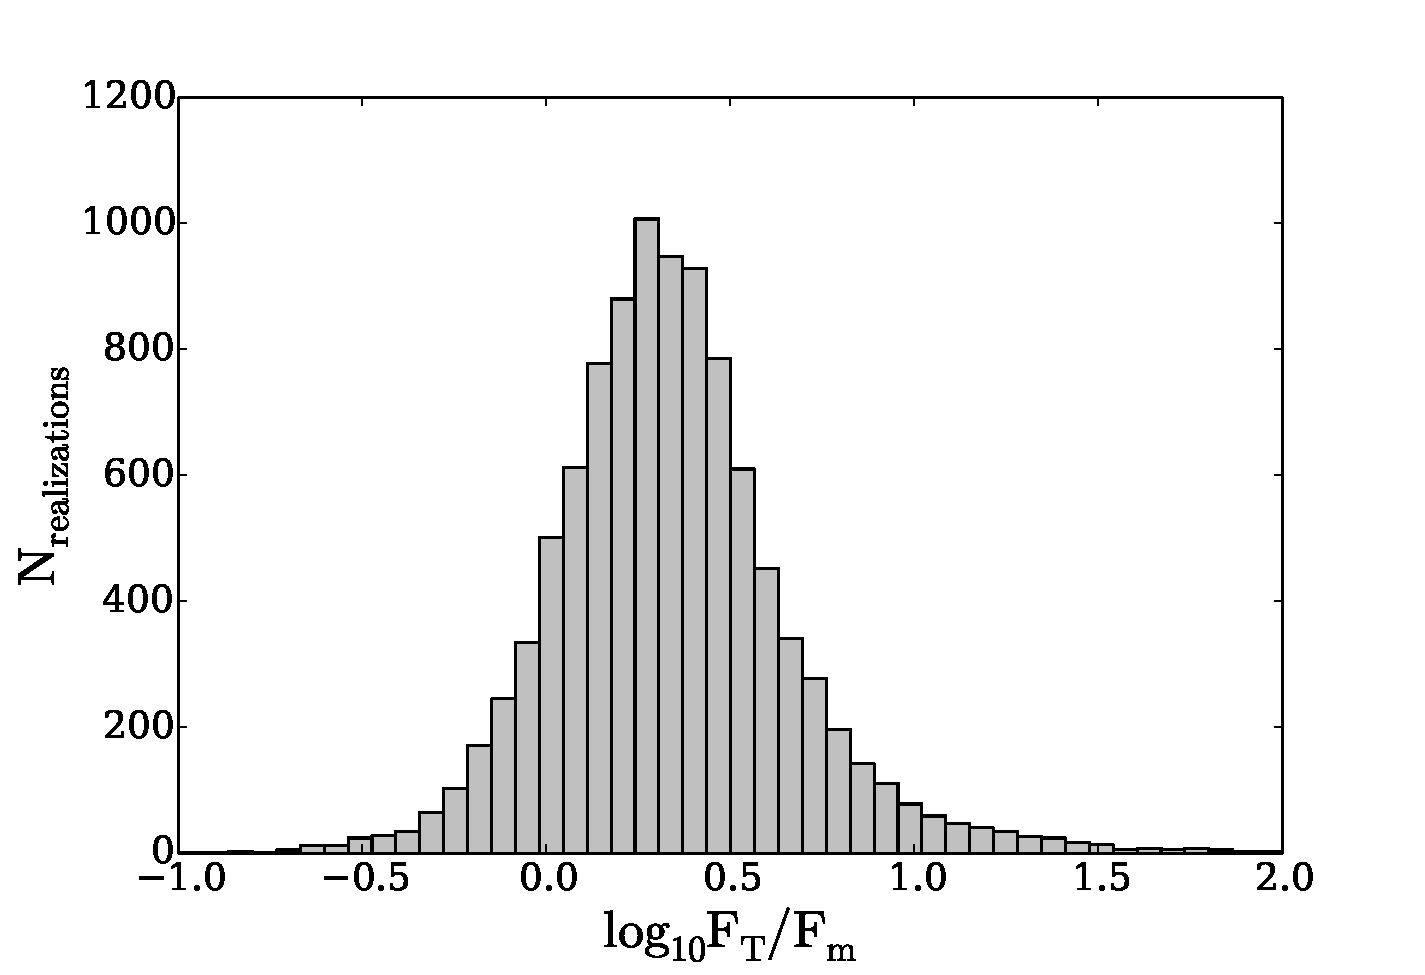
\includegraphics[width=0.8\linewidth,angle=0]{spheres_bulk.pdf}
\caption{\label{fig:sphere_bulk} Frequency of the norm of the total
  force per unit mass produced by a set of identical $N_p$ particles
  homogeneously distributed inside a sphere of radius $R$. This
  corresponds to $10^4$ different realizations of $N_p=10^4$ particles
 each. The values of $F_T$ is normalized to the force per unit mass
 produced by a single particle located at a distance $R_s$ equal to
 the average interparticle separation from the center. \label{fig:sphere_surface}.} 
\end{center}
\end{figure}


5. In the case of the actual large scale matter distribution in the
Universe, galaxies are found to have two distinct characteristics with
respect our toy model. First, the galaxies are not randomly
distributed, but clustered. Second, the galaxies span a wide range of
masses, with less massive galaxies being more common than massive
galaxies. In order to test the influence of these two carachteristics
we use a large comological N-body simulation.[...]

6. The results of the simulation [...] 

\begin{figure}
\begin{center}
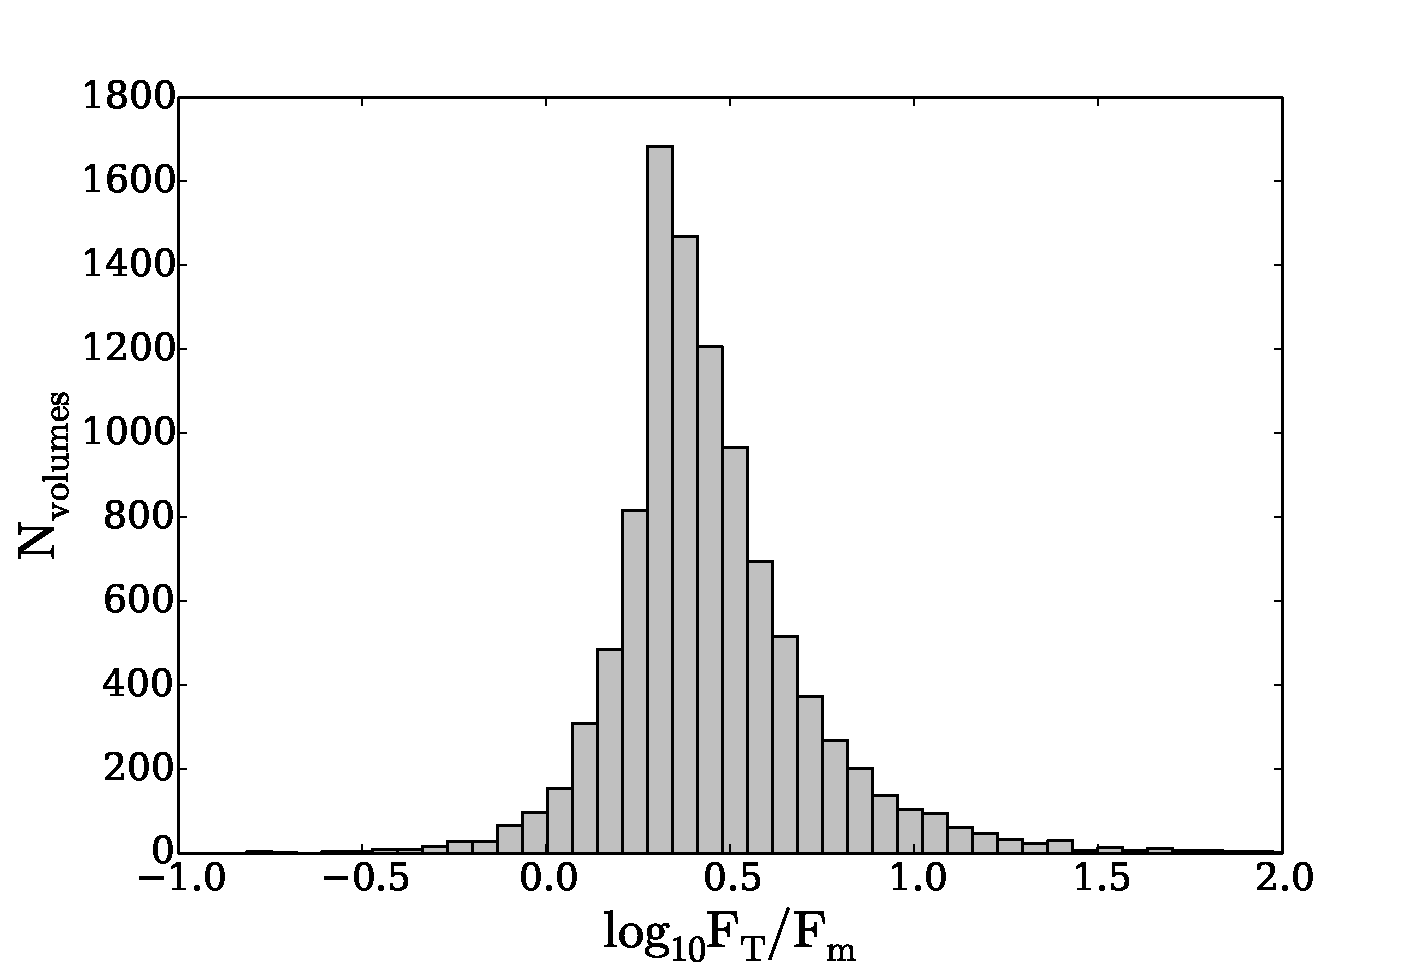
\includegraphics[width=0.8\linewidth,angle=0]{spheres_nbody.pdf}
\caption{\label{fig:sphere_nbody} Frequency of the norm of the total
  force per unit mass produced by a halos inside a spherical volume
  from a cosmological N-body simulation. The radius of the spherical
  region is $300$ $h^{-1}$ Mpc. This corresponds to $10^4$ different volumes 
 The values of $F_T$ are normalized to the force per unit mass
 produced by a single particle located at a distance $R_s$ equal to
 the average interparticle separation from the center and a mass equal
 to the average mass of all halos in the spherical volumne. 
\label{fig:sphere_nbody}.} 
\end{center}
\end{figure}



7. We also consider the variation in the direction of the net force
when the positions of the halos are perturbed within 1 $h^{-1}$ which
is the typical lnghtscale that these objects are expected to travel in
the age of the Universe.


8. The fact that our simple analytical model describes the result
obtained by simulations strenghtens our interpretation on the basis of
fundamental point processes. [...]

9. The velocity of our galaxy in the rest-frame of the cosmic
micriwave background is 627 km
s$^{-1}$. [http://arxiv.org/pdf/1109.3856v1.pdf]. It has been inferred
that the $382$ km s$^{-1}$ are induced by the mass distribution within
$R=30$ $h^{-1}$ Mpc, we call this the local component. This gives a
net result of 382 km s$^{-1}$ that must be induced by the matter
distribution from matter with positions beyond $R$, this is referred
as the tidal component.  Both components, local and tidal, are
pointing in the same direction (??? SURE ??).[...]

10. The effects of the net force imposed by the matter distribution
in the Universe is also in principle detectable in systems isolated 
from massive structures. The most interesting case would be the
kinematic evolution of galaxies located in large scale voids. In these
regions the dominant gravitational interaction would be provided by
the tidal component and not by nearby
structures. [http://adsabs.harvard.edu/abs/2011IJMPS...1...41V] 



11. Possible effects on detailed methods that seek to infer local
density distributions from peculiar velocity measurements. 

12. The physics of this effect are very simple to interpret.




\bibliographystyle{unsrt}
\bibliography{references} 




\end{document}
